\section{PCB Layout and Current Paths}
\label{sec:hw-layout}

The four-layer V1.0 board was arranged to follow the power path. The AC input is on the left, followed by the central charge pump and GaN stage, then the magnetics, rectifier, output, and control sections. The manufactured layout is shown in \Cref{fig:pcb-v1-0-placement-reference,fig:pcb-v1-0-layout-overview}.

\begin{figure}[htbp]
\centering
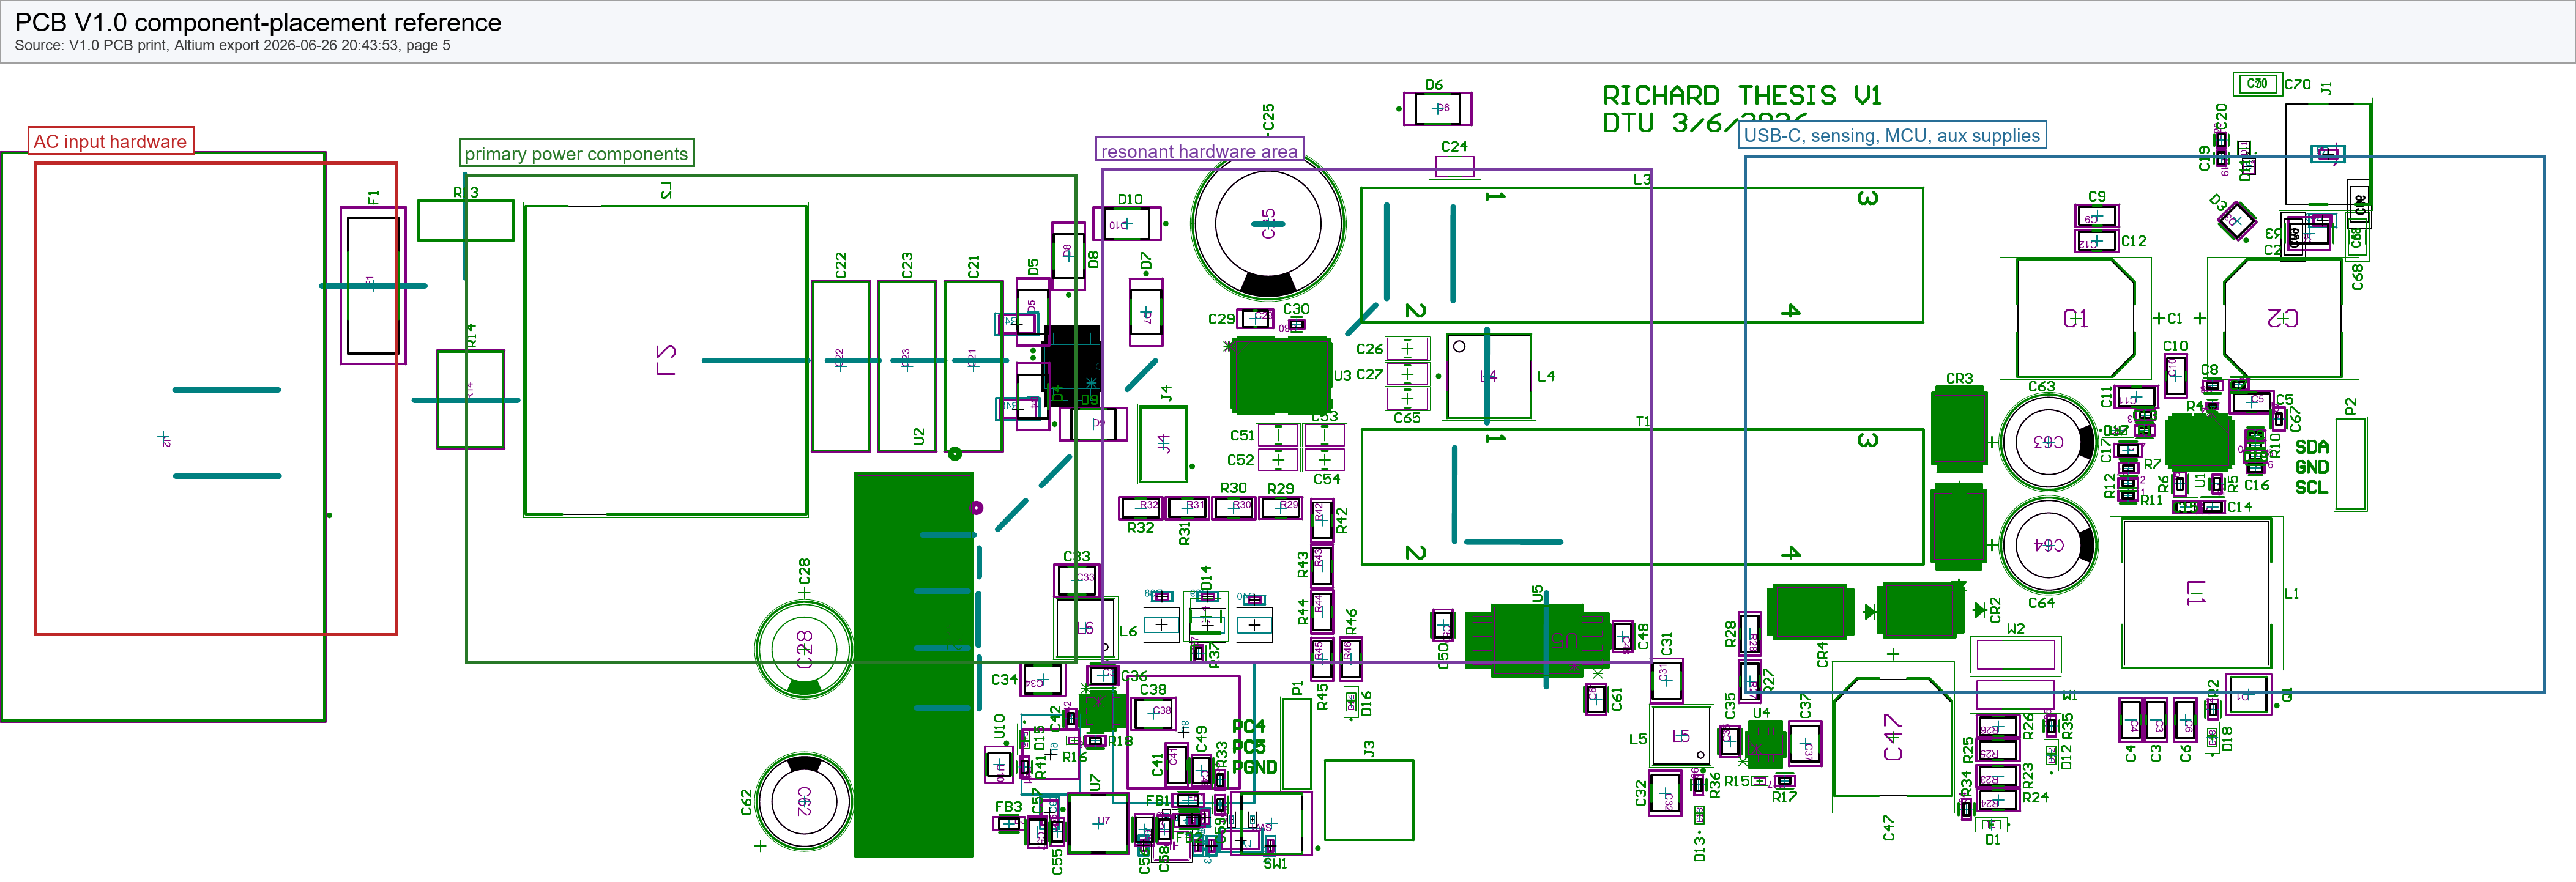
\includegraphics[width=\textwidth]{Pictures/Thesis/07_Hardware/pcb_v1_0_component_placement_reference.png}
\caption{V1.0 component placement. The AC input, high-frequency power stage, magnetics, and output/control circuits are marked.}
\label{fig:pcb-v1-0-placement-reference}
\end{figure}

\begin{figure}[htbp]
\centering
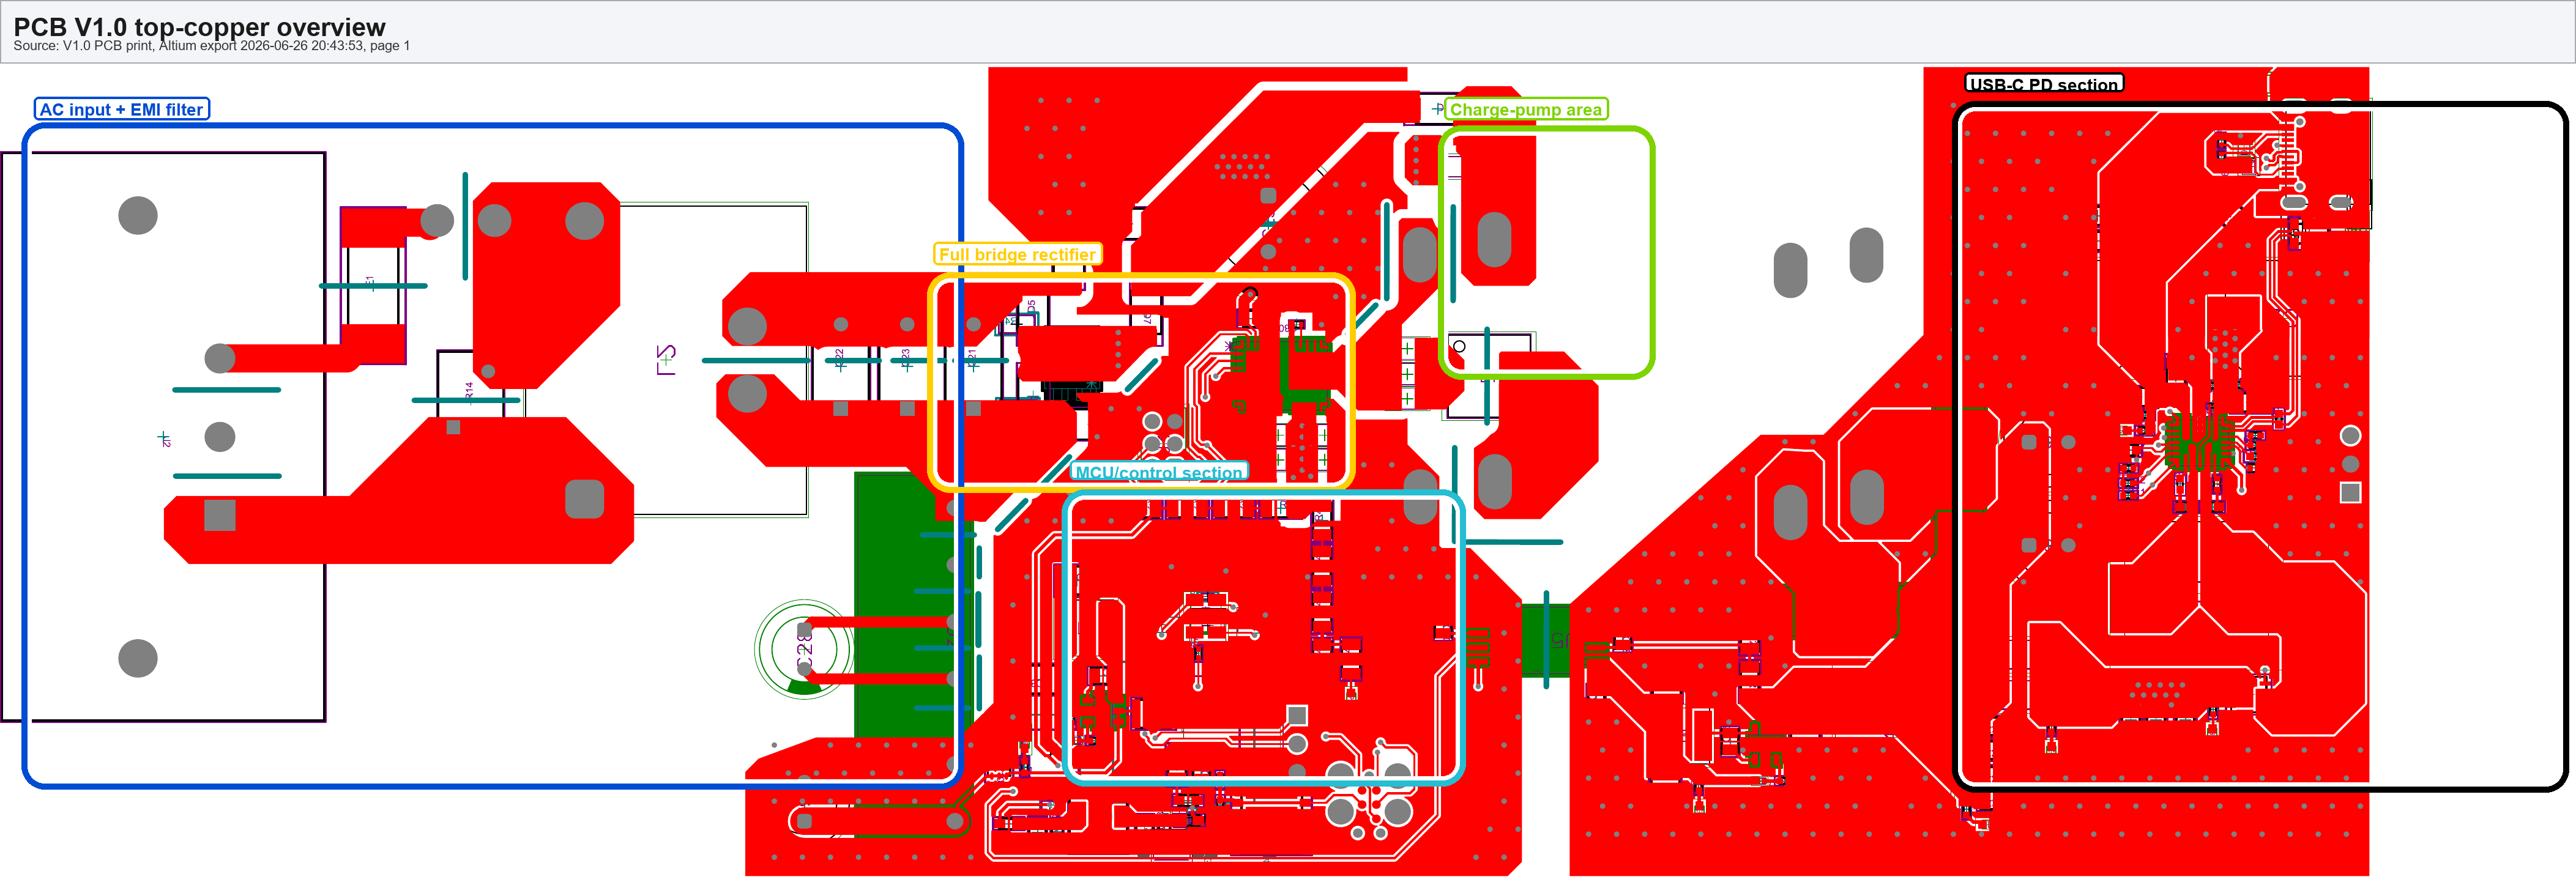
\includegraphics[width=\textwidth]{Pictures/Thesis/07_Hardware/pcb_v1_0_top_copper_overview_annotated_v2.png}
\par\smallskip
\small (a) Top copper and principal component regions.
\par\medskip
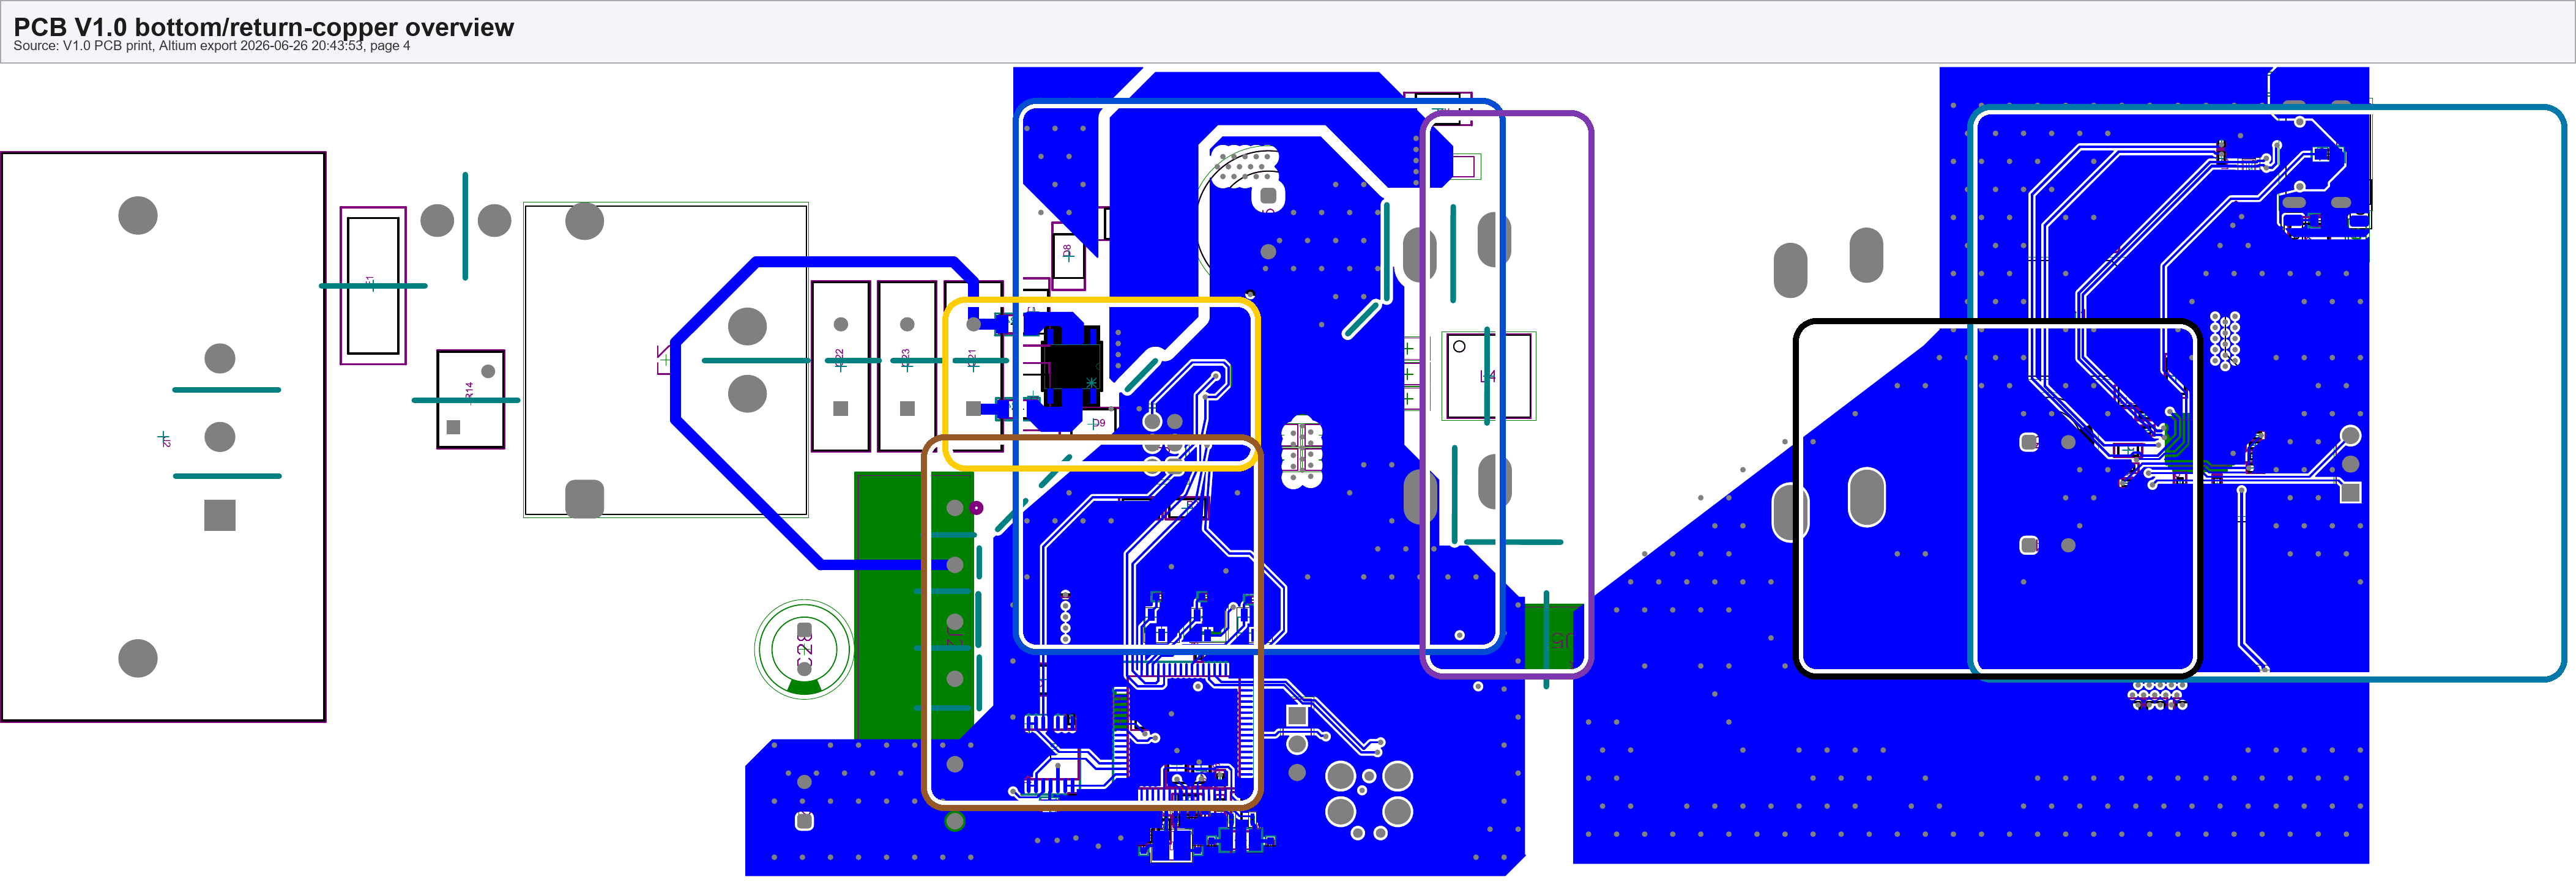
\includegraphics[width=\textwidth]{Pictures/Thesis/07_Hardware/pcb_v1_0_bottom_return_overview_annotated_v2.png}
\par\smallskip
\small (b) Bottom copper and return paths.
\caption{V1.0 top and bottom copper, showing component regions and return paths.}
\label{fig:pcb-v1-0-layout-overview}
\end{figure}

At \SI{1}{\mega\hertz}, parasitic inductance depends on the complete loop. The half-bridge loop closes through its local link decoupling and return. The resonant loop closes through the transformer connections, while the pump capacitor and diodes carry link-charging pulses. Added inductance can change both overshoot and the current available during dead time.

The high-\(dv/dt\) node also couples into nearby copper. Its position relative to the sensing and transformer connections affects analog noise and common-mode current. The return paths must therefore be considered along with the signal traces. These paths are shown in the annotated views. Loop inductance and common-mode capacitance still need to be measured to quantify their contribution.

The final series-inductor connections differ from the original footprint. Their length and support affect the tested tank impedance and must be reproduced along with the component values. The carrier-pin correction showed another layout dependency: the MCU pin on the drawing must support the required timer output.

Clearance of \SI{1}{\milli\metre} and creepage of \SI{3}{\milli\metre} were specified for the relevant nets. The insulation was then checked in the laboratory. A full assessment must also cover the installed transformer, working voltage, material assumptions, and standardized dielectric testing.
